\documentclass[journal]{IEEEtran}

\usepackage{amsmath}
\usepackage{array}
\usepackage{booktabs}
\usepackage{cite}
\usepackage{graphicx}
\usepackage{siunitx}
\usepackage{tikz}
\usepackage{url}
\usepackage{xcolor}
\usetikzlibrary{arrows.meta,calc,fit,patterns,positioning}

\sisetup{
  table-number-alignment=center,
  round-mode=places,
  round-precision=6
}

\newcommand{\rotrng}{RO-TRNG}
\newcommand{\tdc}{TDC}
\newcommand{\spn}{SP800-90B}
\newcolumntype{L}[1]{>{\raggedright\arraybackslash}p{#1}}
\newcommand{\pbad}{$P_\mathrm{bad}$}
\newcommand{\pbal}{$P_\mathrm{balanced}$}
\newcommand{\pcompact}{$P_\mathrm{compact}$}
\newcommand{\pcolumn}{$P_\mathrm{column}$}
\newcommand{\pfar}{$P_\mathrm{far}$}
\newcommand{\psparse}{$P_\mathrm{sparse}$}
\newcommand{\scompact}{$S_\mathrm{compact}$}
\newcommand{\srestart}{$S_\mathrm{restart}$}

\definecolor{boundaryblue}{RGB}{49,94,142}
\definecolor{softblue}{RGB}{223,235,246}
\definecolor{softorange}{RGB}{248,232,210}
\definecolor{softgreen}{RGB}{226,240,226}
\definecolor{softgray}{RGB}{238,238,238}

\begin{document}

\title{A Measurement-Driven Two-Board Case Study of Sampler-Side Entropy Boundaries in Zynq-7020 FPGA RO-TRNGs}

\author{Author Names Withheld for Draft Review}

\maketitle

\begin{abstract}
FPGA ring-oscillator true random number generators are commonly evaluated from oscillator-array structure and final output statistics. This paper reports a two-board Zynq-7020 \rotrng{} case study showing that this boundary can be insufficient: sampler-side physical implementation can substantially reshape measured restart behavior. Continuous-stream placement measurements on the primary board expose a large implementation dependence, from a biased placement with $p_1=0.337316$ and bit min-entropy 0.593606 to a near-balanced placement with $p_1=0.499969$ and bit min-entropy 0.999909. Restart measurements then show that continuous-stream balance is not enough: warmup bytes 8 and 10 trigger fixed-position diagnostic flags, while warmup bytes 11, 12, and 16 do not. The central evidence is a bidirectional sampler-side counterfactual on the primary board, plus a targeted second-board check: imposing the restart-oriented sample-RO lock changes a compact sampler configuration toward biased restart behavior on both boards, with board-specific magnitudes. Pairwise and exact counterfactual \tdc{} diagnostics show small phase correlations under the applied screens, and reduced-XOR controls show that final all64 output can hide biased internal sampler-vector directions through warmup-dependent cancellation. These measurements support a diagnostic claim rather than a certification claim: sampler-side physical implementation is not passive readout in the evaluated implementations and should be included in the measured entropy-source boundary.
\end{abstract}

\begin{IEEEkeywords}
FPGA, ring oscillator, true random number generator, entropy source, placement, restart test, sampler, time-to-digital converter.
\end{IEEEkeywords}

\section{Introduction}

Ring-oscillator true random number generators (\rotrng{}s) are attractive for FPGAs because they can be built from ordinary logic resources and exploit on-chip timing uncertainty as an entropy source \cite{Sunar_2007,Fischer_2008,Wold_2009}. Their measured behavior, however, is inseparable from implementation. Placement, routing, clocking, reset sequencing, sampling, and readout can all affect the final bitstream. For an implemented FPGA \rotrng{}, the measurement problem is therefore not only whether the output stream looks random. It is also where the physical entropy-source boundary should be drawn.

The objective is not to certify a new TRNG architecture, but to diagnose the physical and temporal measurement boundary needed to interpret restart behavior in an implemented FPGA \rotrng{}.

This question matters because a sampler is often treated as a readout mechanism around an oscillator source. That abstraction is useful for design, but it can fail as a measurement boundary. In the measurements reported here, a placement that is near balanced in a continuous stream still shows warmup-dependent fixed-position restart bias. More importantly, small locked changes to the sample-RO physical implementation move restart behavior in both directions: a compact sampler configuration becomes biased when a restart-oriented sample-RO lock is imposed, and the baseline restart configuration is restored near balance when the compact sample-RO lock is imposed. The novelty is not placement dependence alone, but the use of bidirectional sampler-side physical counterfactuals to test the measured entropy-source boundary.

The central question of this paper is:

\begin{quote}
When an FPGA \rotrng{} is evaluated from hardware measurements, must the sampler-side physical implementation be included in the measured entropy-source boundary?
\end{quote}

For the evaluated Zynq-7020 implementations, the answer is yes. The claim is not that all FPGA \rotrng{}s behave identically, nor that the present evidence is a complete \spn{} validation package. The claim is sharper: in these measured implementations, sampler-side physical implementation is not passive readout, and a measurement boundary that excludes it would miss a major observed source of restart-behavior variation under the evaluated protocol.

The contributions are as follows.

\begin{enumerate}
  \item A placement-sensitive continuous-stream characterization showing repeatable output-quality differences across implemented FPGA placements.
  \item A restart and warmup analysis showing that near-balanced continuous-stream statistics do not rule out fixed-position startup bias.
  \item A bidirectional primary-board sampler-side counterfactual, with a targeted second-board check, showing that a sampler-centered physical perturbation can move restart behavior toward biased outcomes and restore near-balanced behavior in the reverse direction on the primary board.
  \item A \tdc{}-assisted diagnostic layer that constrains a simple persistent pairwise hard-locking explanation under the measured conditions.
  \item A reduced-XOR counterfactual analysis showing same-data-RO direction anisotropy, warmup-dependent complement cancellation, line-direction controls, and a second-board mechanism check.
\end{enumerate}

The rest of the paper follows the evidence chain. Section~II summarizes related work and the measurement gap. Section~III describes the implemented system and workflow. Section~IV defines the experimental boundary and analysis rules. Sections~V--IX present continuous-stream placement, restart, sampler-side counterfactual, \tdc{}, and reduced-XOR evidence. Section~X discusses the entropy-source boundary, Section~XI lists limitations and future measurements, and Section~XII concludes.

\section{Background and Measurement Gap}

FPGA \rotrng{}s use oscillator-derived timing uncertainty, sampling logic, and combining or conditioning logic to generate random bits \cite{Sunar_2007,Fischer_2008,Wold_2009,Bochard_2009}. Oscillator-based TRNG work also warns that test-passing streams can contain deterministic or pseudo-random structure unless the source model and sampling assumptions are examined carefully \cite{Baudet_2011,Bochard_2010}. Evaluation may include output statistics, entropy estimates, restart behavior, health-test boundaries, and conditioning documentation \cite{Turan_2018,Lubicz_2015,Lubicz_2024}. Prior work further shows that oscillator-based generators can be sensitive to implementation and environmental conditions, including security-relevant perturbations \cite{Markettos_2009,Fischer_2008}.

Recent FPGA TRNG architecture studies reinforce the implementation theme. Compact multi-RO, RO-PUF/TRNG, and DCM/metastability designs report area, throughput, portability, and platform tradeoffs, and some explicitly evaluate place-and-route dependence as part of the hardware study \cite{Nannipieri_2021,RojasMunoz_2022,Frustaci_2023}. These works motivate careful reporting of FPGA implementation details, but they do not replace a project-specific boundary diagnosis for the particular sampler, restart protocol, and routed implementation studied here.

These foundations cover RO construction, statistical assessment, standards-oriented entropy-source evaluation, active perturbation, and TDC instrumentation. They do not, by themselves, close the implementation-level measurement gap addressed here. A final bitstream is not merely an abstract RTL object; it is a routed physical implementation with local interconnect, resource placement, control logic, and measurement readout. If an evaluation records only final output statistics, it may miss which physical substructure shaped those statistics. Restart-style measurements sharpen the problem because they compare fixed positions across repeated starts and can expose startup-position effects that disappear in aggregate continuous streams \cite{Turan_2018}.

\tdc{} instrumentation provides another diagnostic layer. FPGA \tdc{}s have a substantial instrumentation literature \cite{Jian_Song_2006,Wu_2009,Wu_2012,Wang_2017}, but raw bins are not automatically linear timing measurements. In this work, \tdc{} data are used conservatively: they help test mechanism explanations, especially persistent pairwise hard locking, but they are not used as calibrated picosecond-level jitter metrology.

The distinction of this paper is the sampler-side boundary evidence. Existing \rotrng{} analysis can separate oscillator source, sampler, post-processing, and validation boundary for modeling or certification. The measurements here show that, for the evaluated implementations, treating the sampler side as passive readout is not a safe measurement abstraction. The missing comparison dimension is not simply whether placement affects output quality, but whether a controlled sampler-side physical perturbation changes restart behavior while the measurement boundary is being diagnosed.

\section{Design and Measurement Workflow}

\subsection{Implemented Entropy Source}

The evaluated design is an FPGA \rotrng{} implemented on the Zynq-7020 measurement platform summarized in Table~\ref{tab:setup}. The core entropy RTL contains eight data ROs, a nine-stage sample RO, sampled-data registers, and a final XOR reduction. With the evaluated parameters, the sampled-data vector has 64 bits, formed from eight data ROs sampled across eight sample-RO phases; the final output bit is the XOR reduction of that vector.

Operationally, this paper uses ``measured entropy-source boundary'' to mean the set of physical and temporal implementation elements whose controlled or observed variation can materially change measured output behavior under the evaluated protocol. Under that definition, the boundary is not a certification boundary; it is the boundary needed to interpret the hardware measurements. Figure~\ref{fig:boundary} shows the boundary used here. It includes the data ROs, sample RO, sampled-data registers, sampler-side routing and local implementation, and the restart/warmup/reset timing that directly affects when early samples are taken. FIFO buffering after entropy-bit formation, UART readout, host capture, and offline analysis are outside the entropy source, but they are part of the measurement chain and must be documented for reproducibility.

\begin{figure}[t]
\centering
\resizebox{\columnwidth}{!}{%
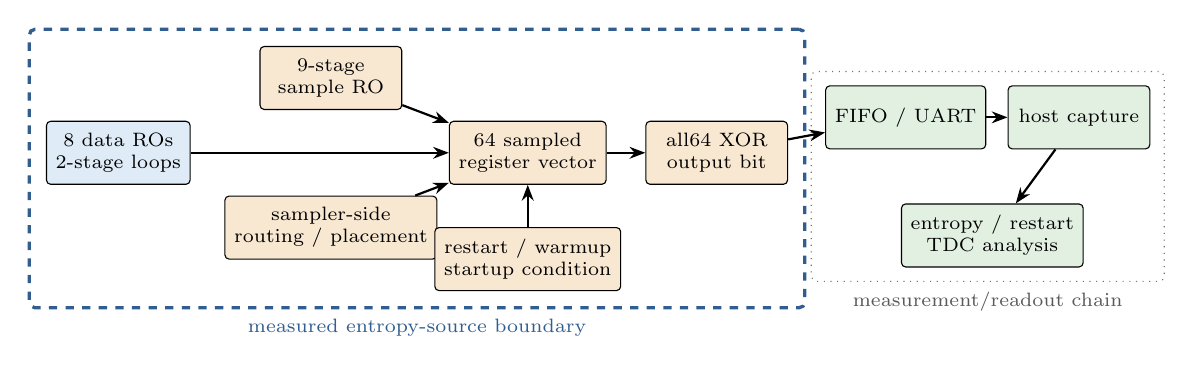
\begin{tikzpicture}[
  font=\scriptsize,
  block/.style={draw, rounded corners=1.5pt, minimum width=18mm, minimum height=8mm, align=center, fill=softgray},
  source/.style={block, fill=softblue},
  sampler/.style={block, fill=softorange},
  readout/.style={block, fill=softgreen},
  arr/.style={-{Stealth[length=2mm]}, thick}
]
\node[source] (data) at (0,0) {8 data ROs\\2-stage loops};
\node[sampler] (sample) at (2.7,0.95) {9-stage\\sample RO};
\node[sampler] (routes) at (2.7,-0.95) {sampler-side\\routing / placement};
\node[sampler] (regs) at (5.2,0) {64 sampled\\register vector};
\node[sampler] (xor) at (7.6,0) {all64 XOR\\output bit};
\node[sampler] (restart) at (5.2,-1.35) {restart / warmup\\startup condition};
\node[readout] (fifo) at (10.0,0.45) {FIFO / UART};
\node[readout] (host) at (12.2,0.45) {host capture};
\node[readout] (analysis) at (11.1,-1.05) {entropy / restart\\TDC analysis};
\draw[arr] (data) -- (regs);
\draw[arr] (sample) -- (regs);
\draw[arr] (routes) -- (regs);
\draw[arr] (restart) -- (regs);
\draw[arr] (regs) -- (xor);
\draw[arr] (xor) -- (fifo);
\draw[arr] (fifo) -- (host);
\draw[arr] (host) -- (analysis);
\node[draw=boundaryblue, dashed, very thick, rounded corners=2pt,
      fit=(data)(sample)(routes)(regs)(xor)(restart), inner sep=6pt,
      label={[font=\scriptsize, text=boundaryblue]below:measured entropy-source boundary}] {};
\node[draw=black!55, dotted, rounded corners=2pt,
      fit=(fifo)(host)(analysis), inner sep=5pt,
      label={[font=\scriptsize, text=black!65]below:measurement/readout chain}] {};
\end{tikzpicture}}
\caption{Operational measured boundary used in this paper. The sampler side, local physical implementation, and restart/warmup/reset timing that directly affects sampling are inside the evaluated entropy-source boundary; post-XOR FIFO buffering, UART, host capture, and offline analysis are measurement/readout elements.}
\label{fig:boundary}
\end{figure}

\subsection{Evidence Workflow}

The workflow is organized as a causal measurement chain rather than a collection of unrelated tests. Figure~\ref{fig:workflow} summarizes the order used in the results: placement first establishes implementation sensitivity; restart exposes fixed-position startup bias; sampler-side counterfactuals test the boundary; \tdc{} diagnostics constrain one simple mechanism explanation; and reduced-XOR counterfactuals show same-data-RO direction anisotropy and warmup-dependent cancellation in the final output. The final node is the boundary conclusion, not a standalone performance claim.

\begin{figure}[t]
\centering
\resizebox{\columnwidth}{!}{%
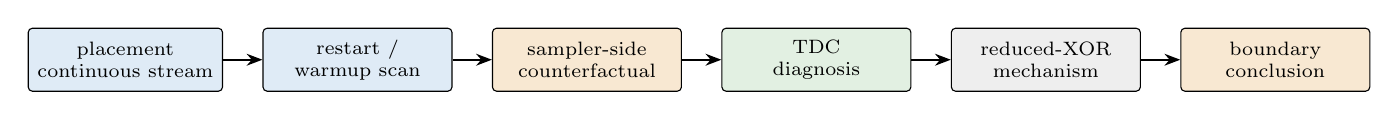
\begin{tikzpicture}[
  font=\scriptsize,
  flowstep/.style={draw, rounded corners=1.5pt, minimum width=24mm, minimum height=8mm, align=center, fill=softgray},
  arr/.style={-{Stealth[length=2mm]}, thick}
]
\node[flowstep, fill=softblue] (p) {placement\\continuous stream};
\node[flowstep, fill=softblue, right=5mm of p] (r) {restart /\\warmup scan};
\node[flowstep, fill=softorange, right=5mm of r] (s) {sampler-side\\counterfactual};
\node[flowstep, fill=softgreen, right=5mm of s] (t) {TDC\\diagnosis};
\node[flowstep, fill=softgray, right=5mm of t] (x) {reduced-XOR\\mechanism};
\node[flowstep, fill=softorange, right=5mm of x] (b) {boundary\\conclusion};
\draw[arr] (p) -- (r);
\draw[arr] (r) -- (s);
\draw[arr] (s) -- (t);
\draw[arr] (t) -- (x);
\draw[arr] (x) -- (b);
\end{tikzpicture}}
\caption{Evidence workflow. The sampler-side counterfactual is the central boundary test; the other measurements establish context, constrain mechanisms, and explain how final-output statistics can hide internal structure.}
\label{fig:workflow}
\end{figure}

\section{Experimental Setup and Analysis Rules}

Table~\ref{tab:setup} records the platform and capture configuration that are fixed or recoverable from archived measurement artifacts. Values that vary across experiments are reported at the result table rather than treated as a single global constant.

\begin{table}[t]
\centering
\caption{Experimental platform and capture configuration.}
\label{tab:setup}
\footnotesize
\begin{tabular}{@{}L{0.35\columnwidth}L{0.57\columnwidth}@{}}
\toprule
Item & Evaluated configuration \\
\midrule
Board scope & Primary Zynq-7020 lab board, hardware root \texttt{20260511\_fpga1\_board1}; targeted second-board checks, hardware root \texttt{20260529\_fpga1\_board2} \\
FPGA part & \texttt{xc7z020clg400-2} \\
Tool flow & Vivado 2023.2 in-memory build scripts \\
System clock & Single-ended board clock through clock wizard; internal UART/control clock 200 MHz \\
UART capture & 115200 baud, 8N1, no flow control; host logs use COM3 \\
Entropy RTL & 8 data ROs, 2 data-RO stages, 9 sample-RO stages \\
Sampled vector & 64 sampled bits per output reduction \\
Output combining & XOR reduction of the sampled-data vector \\
Restart rows & 1000 rows in the restart/counterfactual artifacts used here \\
Restart body & 125 packed bytes for 1000 bit positions in the bit-symbol restart rows used here \\
Restart timing & 200000 hold cycles and 200000 settle cycles at the 200 MHz control clock in the auto-restart RTL \\
Warmup unit & FIFO output bytes discarded after settle and before recording the row body \\
Entropy tools & NIST EntropyAssessment non-IID and restart tools on prepared bit-symbol inputs \\
\tdc{} windows & 12 pair captures, 16 windows per capture; packet-offset lag scan from $-8$ to $+8$ \\
Repeats & 10 MiB continuous-stream, 5 MiB, 20 MiB, and counterfactual repeats where listed in the measurement artifacts \\
\bottomrule
\end{tabular}
\end{table}

\subsection{Diagnostic Use of Restart Statistics}

The restart analysis is used diagnostically: it asks whether fixed output positions repeat too often across restarts under the evaluated implementation and warmup setting. It is not used as a complete \spn{} validation. The 1000-row restart body follows the restart input shape used by the local \texttt{ea\_restart} flow, not an argument that 1000 rows alone is sufficient for certification.

For the 1000-by-125-byte bit-symbol restart rows, each row records 125 packed bytes and is expanded row-preservingly into 1000 fixed bit-symbol positions. For fixed bit position $j$, let $n_j$ be the number of one bits across the 1000 restart rows and define
\begin{equation}
  x_j = \max(n_j, 1000-n_j).
\end{equation}
The reported ``Worst $x$'' is $\max_j x_j$. The archived analysis also counts fixed positions whose $x_j$ exceeds the applicable \texttt{ea\_restart} cutoff derived from the corresponding non-IID entropy estimate. Table~\ref{tab:warmup} reports the cutoff, maximum count, and resulting diagnostic outcome to keep the table compact; the diagnostic still inspects many fixed positions jointly and is not a collection of independent single-position claims. For the \pbal{} inputs, the archived experiment logs report $H_I=0.902345$ and $X_\mathrm{cutoff}=605$ for the MSB bit-symbol route, and $H_I=0.828444$ and $X_\mathrm{cutoff}=632$ for the LSB route. Table~\ref{tab:warmup} displays the MSB-route cutoff; the LSB route was also checked in the archived restart runs. Overall $p_1$ and fixed-position diagnostic outcome can therefore disagree: a dataset can remain close to $p_1=0.5$ overall while one or more fixed startup positions repeat too often across restarts.

For pairwise \tdc{} analysis, a strong-lock window is a conservative diagnostic flag with maximum absolute lagged phase correlation at or above 0.5 in the packet-offset lag scan from $-8$ to $+8$. This empirical threshold is not a standards definition; it is used only to test whether the selected captures support a simple persistent pairwise hard-locking explanation.

\section{Placement-Sensitive Continuous-Stream Characterization}

Table~\ref{tab:placement} summarizes representative 10 MiB continuous-stream captures from the placement study. The contrast between \pbad{} and \pbal{} is the simplest entry point. In the 10 MiB rows, \pbad{} has $p_1=0.337316$, absolute bias 0.162684, and bit min-entropy 0.593606. In contrast, \pbal{} has $p_1=0.499969$, absolute bias $3.14355\times 10^{-5}$, and bit min-entropy 0.999909.

The table also shows why balance alone is insufficient. The same-column placement is near balanced by $p_1$ and bit min-entropy, but its adjacent-equal ratio differs from the strongest placements. This motivates the restart and mechanism measurements: a single continuous-stream statistic cannot define the physical entropy-source boundary.

\begin{table*}[t]
\centering
\caption{Representative 10 MiB continuous-stream placement statistics. Artifact IDs preserve traceability to the experiment logs.}
\label{tab:placement}
\scriptsize
\begin{tabular}{llrrrrrl}
\toprule
Paper condition & Artifact ID & Bytes & $p_1$ & Abs. bias & Bit min-H & Adjacent equal & Reading \\
\midrule
\pcompact{} & compact & 10 MiB & 0.499948 & 0.000052 & 0.999850 & 0.499939 & near-balanced reference \\
\pbal{} & random3 & 10 MiB & 0.499969 & 0.000031 & 0.999909 & 0.500072 & near-balanced stream \\
\pcolumn{} & same\_column & 10 MiB & 0.499930 & 0.000070 & 0.999799 & 0.505980 & balanced $p_1$ with structural warning \\
\pfar{} & far & 10 MiB & 0.491508 & 0.008492 & 0.975703 & 0.500726 & biased stream \\
\psparse{} & sparse & 10 MiB & 0.464350 & 0.035650 & 0.900637 & 0.506596 & stronger bias and structure \\
\pbad{} & random1 & 10 MiB & 0.337316 & 0.162684 & 0.593606 & 0.556740 & poor placement \\
\bottomrule
\end{tabular}
\end{table*}

Available repeats support placement-level consistency for the current dataset. The summarized measurements report a maximum 10 MiB/repeat bit-min-entropy mean delta of 0.00841786 among paired placement rows. The continuous-stream placement matrix itself remains primary-board evidence rather than a cross-board placement ranking, but it supports treating the placement differences as measured implementation behavior in the evaluated experiment.

\section{Restart and Warmup Characterization}

\subsection{Continuous-Stream Entropy Is Not Enough}

Table~\ref{tab:sp800summary} shows non-IID entropy-assessment summaries for selected bit-symbol inputs. \pbal{} has a higher non-IID $H_\mathrm{original}$ than \pbad{} in the 8,000,000-symbol summary, consistent with its strong continuous-stream balance. However, restart measurements reveal warmup-dependent fixed-position bias for \pbal{}. The relevant measurement question is therefore not simply which continuous stream looks best, but whether the implemented source remains stable under repeated startup measurements.

\begin{table}[t]
\centering
\caption{Selected non-IID entropy-assessment summaries.}
\label{tab:sp800summary}
\scriptsize
\begin{tabular}{llcc}
\toprule
Paper condition & Artifact ID & Symbols & $H_\mathrm{original}$ \\
\midrule
reference & original\_fpga1\_run01 & 8,000,000 & 0.877727 \\
\pbad{} & random1\_run01 & 8,000,000 & 0.389520 \\
\pbal{} & random3\_run01 & 8,000,000 & 0.902345 \\
\bottomrule
\end{tabular}
\end{table}

\subsection{Warmup Transition}

Table~\ref{tab:warmup} gives the \pbal{} restart warmup transition. Under the evaluated board, placement, and auto-stream restart protocol, no-warmup, warmup 8, and warmup 10 trigger fixed-position diagnostic flags, while warmup settings 11, 12, and 16 do not. Repeated warmup scans place the observed transition at $10 < \texttt{WARMUP\_BYTES} \le 11$, with warmup 11 still a boundary observation rather than a large-margin engineering rule.

\begin{table}[t]
\centering
\caption{\pbal{} restart warmup transition. ``Flag'' means at least one fixed bit position exceeds the displayed MSB-route cutoff $X_\mathrm{cutoff}=605$; archived LSB-route checks use $X_\mathrm{cutoff}=632$.}
\label{tab:warmup}
\scriptsize
\begin{tabular}{rrrrrl}
\toprule
Warmup & Overall $p_1$ & Route & Cutoff & Worst $x$ & Diagnostic outcome \\
\midrule
0  & 0.497933 & MSB & 605 & 685 & flag \\
8  & 0.374385 & MSB & 605 & 721 & flag \\
10 & 0.415017 & MSB & 605 & 650 & flag \\
11 & 0.469088 & MSB & 605 & 583 & no flag \\
12 & 0.499478 & MSB & 605 & 562 & no flag \\
16 & 0.499126 & MSB & 605 & 549 & no flag \\
\bottomrule
\end{tabular}
\end{table}

The transition is important because the continuous-stream \pbal{} row is near ideal, yet early restart positions remain sensitive to the warmup setting. Thus, the restart result does not merely add another performance number; it identifies a measurement mode in which the physical sampling boundary matters. The repeated warmup-10 flagged outcomes and warmup-11 no-flag outcomes support a narrow measured transition, but they should not be generalized as a universal warmup threshold across boards, placements, PVT conditions, or tool runs.

\section{Sampler-Side Counterfactuals}

The central evidence for the entropy-boundary claim is the sampler-side counterfactual loop in Table~\ref{tab:samplero}. The compact diagnostic RTL configuration is the restart configuration used to isolate a compact sampler passband. The baseline restart RTL configuration is the auto-stream restart configuration used in the 1000-row restart measurements. The sample-RO locks are defined by explicit LOC/BEL constraints: \scompact{} uses the compact sample-RO placement and \srestart{} uses the restart-oriented sample-RO placement from the baseline restart constraint set. The term \srestart{} is a placement label, not a formal-verification claim.

\begin{table*}[t]
\centering
\caption{Bidirectional sampler-side counterfactual evidence. Rows are representative run-level measurements; archive identifiers are omitted from the main table and retained in the experiment logs.}
\label{tab:samplero}
\scriptsize
\begin{tabular}{llllrrrL{0.22\textwidth}}
\toprule
Direction & RTL configuration & Sample-RO lock & Warmup & $p_1$ & Min-H & Worst $x$ & Outcome \\
\midrule
baseline & compact diagnostic & \scompact{} & 4  & 0.498297 & 0.995095 & 555 & no diagnostic flag \\
baseline & compact diagnostic & \scompact{} & 5  & 0.498316 & 0.995149 & 549 & no diagnostic flag \\
baseline & compact diagnostic & \scompact{} & 11 & 0.498148 & 0.994666 & 548 & no diagnostic flag \\
forward & compact diagnostic & \srestart{} & 4 & 0.376651 & 0.681888 & 884 & diagnostic flag with bias \\
forward & compact diagnostic & \srestart{} & 4 & 0.378757 & 0.686770 & 752 & reproduced diagnostic flag \\
forward & compact diagnostic & \srestart{} & 5 & 0.373430 & 0.674452 & 757 & diagnostic flag with bias \\
forward & compact diagnostic & \srestart{} & 5 & 0.373541 & 0.674708 & 792 & reproduced diagnostic flag \\
forward & compact diagnostic & \srestart{} & 5 & 0.371751 & 0.670592 & 745 & reproduced diagnostic flag \\
forward & compact diagnostic & \srestart{} & 11 & 0.464819 & 0.901901 & 576 & residual bias \\
reverse & baseline restart & \scompact{} & 4 & 0.499419 & 0.998325 & 552 & near-balanced behavior restored \\
reverse & baseline restart & \scompact{} & 4 & 0.499754 & 0.999290 & 552 & reproduced restoration \\
reverse & baseline restart & \scompact{} & 4 & 0.499432 & 0.998362 & 560 & reproduced restoration \\
\bottomrule
\end{tabular}
\end{table*}

\begin{table*}[t]
\centering
\caption{Archived repeat summary for the sampler-side counterfactual rows. Table~\ref{tab:samplero} lists representative run-level measurements; this table summarizes all currently archived repeats for the listed condition and warmup. Min-H is the bit min-entropy computed from each row's overall $p_1$ when the source summary did not store it explicitly.}
\label{tab:counterrepeat}
\scriptsize
\begin{tabular}{llrrrrrL{0.23\textwidth}}
\toprule
Case & Warmup & $n$ & Mean $p_1$ & Std. $p_1$ & Min. Min-H & Max worst $x$ & Repeat coverage \\
\midrule
compact baseline & 4  & 3 & 0.498812 & 0.000450 & 0.995095 & 562 & three independent captures \\
compact baseline & 5  & 2 & 0.498796 & 0.000679 & 0.995149 & 549 & two independent captures \\
compact baseline & 11 & 2 & 0.498287 & 0.000196 & 0.994666 & 548 & two independent captures \\
forward fail & 4  & 3 & 0.377401 & 0.001176 & 0.681888 & 884 & three archived implementation repeats \\
forward fail & 5  & 3 & 0.372907 & 0.001003 & 0.670592 & 792 & three independent captures \\
forward fail & 11 & 2 & 0.462977 & 0.002605 & 0.892004 & 588 & two independent captures \\
reverse repair & 4  & 3 & 0.499535 & 0.000190 & 0.998325 & 560 & three independent captures \\
\bottomrule
\end{tabular}
\end{table*}

\begin{table}[t]
\centering
\caption{Targeted second-board sampler counterfactual check.}
\label{tab:board2counter}
\scriptsize
\resizebox{\columnwidth}{!}{%
\begin{tabular}{llrrrl}
\toprule
Sample-RO lock & Warmup & $p_1$ & Min-H & Worst $x$ & Reading \\
\midrule
\scompact{}  & 4 & 0.493833 & 0.982315 & 571 & compact reference \\
\srestart{}  & 4 & 0.453148 & 0.870778 & 713 & shifted toward biased restart behavior \\
\scompact{}  & 5 & 0.517910 & 0.949227 & 572 & compact reference \\
\srestart{}  & 5 & 0.447170 & 0.855092 & 648 & shifted toward biased restart behavior \\
\bottomrule
\end{tabular}}
\end{table}

The forward direction on the primary board shows that a compact diagnostic configuration that is near balanced with \scompact{} becomes biased when \srestart{} is imposed. The reverse direction prevents the result from being read as a one-way artifact of the diagnostic configuration: the baseline restart configuration is restored near balance when \scompact{} is imposed. Table~\ref{tab:samplero} is run-level counterfactual diagnostic evidence rather than a balanced statistical repeatability study, and Table~\ref{tab:counterrepeat} makes the uneven archived repeat coverage explicit. Where same-condition repeats are currently available, the sign of the effect is stable: the three-row forward warmup-4 and warmup-5 groups remain biased, the three-row reverse warmup-4 group remains near balanced, and the three-row compact-baseline warmup-4 group remains near balanced. The compact baseline warmup-5 and warmup-11 points and the forward warmup-11 point still have two runs each, so these summaries should not be read as a complete repeatability study.

The targeted second-board check in Table~\ref{tab:board2counter} reproduces the direction of the sampler-lock effect without reproducing the exact primary-board magnitudes. At warmup 4, changing from \scompact{} to \srestart{} moves $p_1$ from 0.493833 to 0.453148 and raises the worst fixed-position count from 571 to 713; at warmup 5, it moves $p_1$ from 0.517910 to 0.447170 and raises worst $x$ from 572 to 648. This supports the boundary claim across a second physical board while also showing that the signed magnitude and diagnostic margin are board-specific measurements, not universal constants.

The intended constraint change is localized to explicit sample-RO LOC/BEL constraints, with the same data-RO and sampler-register constraint base retained for the locked variants. The implemented perturbation should therefore be interpreted as a sampler-centered physical perturbation with entropy-source-local routed-network residuals, not as a claim that only three LUT delays changed. Because Vivado may still alter surrounding routes, delays, and neighborhood implementation, the result is evidence that sampler-side physical implementation and local routed context reshape restart behavior rather than proof that no other physical element changed. We therefore separate two uses of the counterfactuals: the same-RTL forward comparisons provide the strongest implementation-locality evidence, while the reverse repair rows provide behavior-level bidirectional evidence but are not used as a clean locality proof.

As a route-variance control, we also rebuilt the same compact-diagnostic warmup-4 pair using Vivado \texttt{Explore} directives for the \texttt{place\_design}, \texttt{phys\_opt\_design}, and \texttt{route\_design} stages. The behavioral split persisted: the compact-lock build remained near balanced ($p_1=0.496761$, Min-H 0.990684, worst $x=560$), while the restart-oriented sample-RO lock remained biased ($p_1=0.375294$, Min-H 0.678751, worst $x=796$). This directive-controlled check reduces the chance that the forward counterfactual is only one default implementation accident, while retaining the same route-residual limitation discussed below.

Table~\ref{tab:implsummary} adds implementation traceability for representative warmup-4 locked variants. The compact diagnostic baseline and the forward counterfactual share the same RTL top and differ in the placement XDC used for the sample-RO lock. The reverse counterfactual uses the baseline restart RTL configuration and the compact sample-RO lock. All three representative bitstreams are fully routed with no routing errors and meet the reported timing constraints. The resource and power numbers are not used as causal proof; they document that the compared implementations are small, routed, and reproducible enough for the counterfactual result to be audited.

\begin{table*}[t]
\centering
\caption{Implementation traceability for representative sampler-side counterfactual bitstreams.}
\label{tab:implsummary}
\scriptsize
\begin{tabular}{llllrrrrll}
\toprule
Variant & RTL configuration & Sample lock & Warmup & WNS & LUT & FF & Power & Routed & Intended constraint change \\
\midrule
baseline & compact diagnostic & \scompact{} & 4 & 0.712 & 350 & 364 & 0.225 W & yes, 0 errors & compact sample-RO lock \\
forward & compact diagnostic & \srestart{} & 4 & 0.638 & 350 & 364 & 0.224 W & yes, 0 errors & 3 listed sample-RO LUT LOC/BEL differences \\
reverse & baseline restart & \scompact{} & 4 & 0.534 & 346 & 363 & 0.223 W & yes, 0 errors & compact sample-RO lock in baseline restart top \\
\bottomrule
\end{tabular}
\end{table*}

Table~\ref{tab:routedaudit} summarizes a routed locality audit extracted from the routed DCPs. The strongest physical-locality comparison is the same-RTL forward warmup-4 pair: tracked data-RO cells and sampled-data registers keep their LOC/BEL assignments, while the sample-RO cells change by 2/9 LOC and 3/9 BEL entries. The route audit still reports changed data-RO and sample-RO net routes, so the evidence is not a sample-RO-only proof. Instead, it supports the bounded claim that the measured boundary includes a sampler-centered physical perturbation with entropy-source-local routed-network residuals.

\begin{table*}[t]
\centering
\caption{Routed locality audit for sampler-side counterfactuals. Cell entries report LOC/BEL changes among common named cells. Route entries report common nets whose routed path changed.}
\label{tab:routedaudit}
\scriptsize
\begin{tabular}{@{}L{0.23\textwidth}L{0.28\textwidth}L{0.23\textwidth}L{0.16\textwidth}@{}}
\toprule
Comparison & Cell-placement changes & Routed-net changes & Manuscript role \\
\midrule
Forward W4, compact diagnostic: \scompact{} to \srestart{} & data-RO: 0/16 LOC, 0/16 BEL; sampled registers: 0/64 LOC, 0/64 BEL; sample RO: 2/9 LOC, 3/9 BEL & data-RO nets: 34/64; sample-RO nets: 18/36; sampled-data nets: 3/64 & Strongest locality evidence; same RTL, sample-RO cell perturbation, routed-network residual remains \\
Directive W4, compact diagnostic, Explore directives: \scompact{} to \srestart{} & data-RO: 0/16 LOC, 0/16 BEL; sampled registers: 0/64 LOC, 0/64 BEL; sample RO: 2/9 LOC, 3/9 BEL & data-RO nets: 34/64; sample-RO nets: 18/36; sampled-data nets: 9/64 & Route-variance control; forward behavior persists under Explore directives \\
Forward W5, compact diagnostic: \scompact{} to \srestart{} & data-RO: 0/16 LOC, 0/16 BEL; sampled registers: 0/64 LOC, 0/64 BEL; sample RO: 2/9 LOC, 3/9 BEL & data-RO nets: 32/64; sample-RO nets: 18/36; sampled-data nets: 10/64 & Repeat implementation check for the forward locality pattern \\
Reverse W4, baseline restart: \srestart{} to \scompact{} & data-RO: 16/16 LOC, 12/16 BEL; sampled registers: 64/64 LOC, 63/64 BEL; sample RO: 2/9 LOC, 3/9 BEL & data-RO nets: 64/64; sample-RO nets: 36/36; sampled-data nets: 64/64 & Behavior-level repair evidence; broader physical perturbation, not locality proof \\
\bottomrule
\end{tabular}
\end{table*}

Figure~\ref{fig:samplerlock} shows the locked sample-RO assignments used for the physical perturbation. The archived XDC and passband notes list three changed sample-RO LUT assignments: \texttt{RO\_SAMPLE\_NAND}, \texttt{RO\_SAMPLE\_LOOP[1]}, and \texttt{RO\_SAMPLE\_LOOP[7]}. The build manifests record the target top module, part, placement XDC, warmup parameter, and Vivado 2023.2 flow; routed-status, timing, utilization, and power reports are the source for Table~\ref{tab:implsummary}. The routed audit also extracted related nets, PIPs, and Vivado net-delay summaries. Those summaries show route-level delay residuals in RO-related nets while the sampled-data input-delay summary is nearly unchanged. This reinforces the interpretation above: sampled-register endpoints are nearly unchanged in placement and summarized input delay, but route changes remain in the entropy-source-local network.

The older broad routed-cell diff between the formal auto and compact warmup-4 builds reports no LOC changes for named entropy-source data-RO cells (0/48) or sampled-data registers (0/64), and sample-RO changes of 2/27 LOC and 3/27 BEL entries, but it also reports many FIFO, control, and UART cell movements. The RTL dataflow helps interpret this result. FIFO and UART logic do not feed a data value back into \texttt{sampled\_data} or \texttt{rand\_bit}; \texttt{tx\_ready} controls readout progress, not the construction of the entropy bit. However, FIFO status and the top-level FSM define drain, warmup, and send timing, so readout/control movement is still a measurement-chain confounder to document. It is not evidence that the entire bitstream should be included inside the entropy-source boundary.

\begin{figure}[t]
\centering
\resizebox{\columnwidth}{!}{%
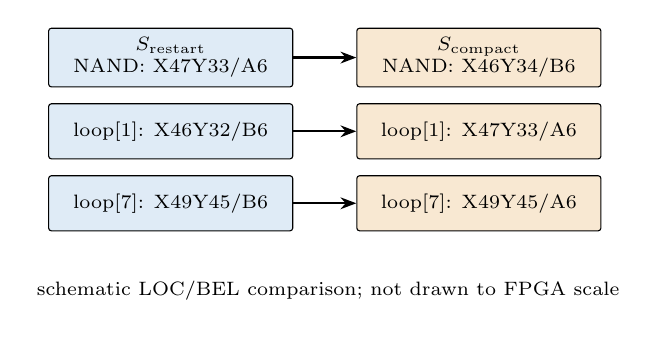
\begin{tikzpicture}[
  font=\scriptsize,
  cell/.style={draw, rounded corners=1pt, minimum width=31mm, minimum height=7mm, align=center},
  arr/.style={-{Stealth[length=2mm]}, thick}
]
\node[cell, fill=softblue] (f1) {\srestart{}\\NAND: X47Y33/A6};
\node[cell, fill=softblue, below=2mm of f1] (f2) {loop[1]: X46Y32/B6};
\node[cell, fill=softblue, below=2mm of f2] (f3) {loop[7]: X49Y45/B6};
\node[cell, fill=softorange, right=8mm of f1] (c1) {\scompact{}\\NAND: X46Y34/B6};
\node[cell, fill=softorange, below=2mm of c1] (c2) {loop[1]: X47Y33/A6};
\node[cell, fill=softorange, below=2mm of c2] (c3) {loop[7]: X49Y45/A6};
\draw[arr] ($(f1.east)+(0,0)$) -- (c1.west);
\draw[arr] ($(f2.east)+(0,0)$) -- (c2.west);
\draw[arr] ($(f3.east)+(0,0)$) -- (c3.west);
\node[align=center, below=5mm of f3, xshift=20mm] {schematic LOC/BEL comparison; not drawn to FPGA scale};
\end{tikzpicture}}
\caption{Sample-RO lock schematic for the counterfactual. Only the listed sample-RO LUT assignments are the intended constraint perturbation in this comparison; implemented local routing and neighborhood effects may still vary.}
\label{fig:samplerlock}
\end{figure}

\section{TDC-Assisted Mechanism Diagnosis}

\subsection{Pairwise TDC Dynamics}

The \tdc{} evidence is not used to prove the root cause of the sampler-side counterfactual. It has a narrower role: rejecting an overly simple mechanism explanation in which the observed restart behavior is attributed only to persistent pairwise hard locking between oscillator pairs. Under the selected pair captures, the \tdc{} measurements do not support that explanation as the dominant mechanism. A phase-correlation value here denotes the absolute correlation between packetized \tdc{} phase sequences within an analysis window. A best-lag value is the largest such magnitude found over packet offsets from $-8$ to $+8$. Across 12 pair captures and 16 windows per capture, the summary reports zero strong-lock windows. The maximum reported small-lag or best-lag absolute correlation is about 0.031783.

An additional exact counterfactual \tdc{} check places the \tdc{} sample-RO lane at the same \scompact{} and \srestart{} LOC/BEL assignments used in Table~\ref{tab:samplero}, while holding the measured data-RO lane at data\_ro0. With warmup-4 reset-aligned captures of 32768 packets per variant, the \scompact{} and \srestart{} runs report phase correlations of 0.004300 and 0.011762, respectively; a 16-window lag scan over $-8$ to $+8$ packets gives zero strong-lock windows for both, with maximum best-lag magnitudes about 0.059012 and 0.057888. This result does not explain the counterfactual by itself, but it further constrains a simple pairwise hard-locking explanation for the observed restart bias. A second-board exact \tdc{} repeat gives the same negative-mechanism reading for direct phase correlation: for data\_ro0, \scompact{} and \srestart{} phase correlations are 0.004264 and 0.008195; for data\_ro3, they are 0.000058 and $-0.001232$, with zero packet sequence gaps in all four 32768-packet captures.

\begin{table*}[t]
\centering
\caption{\tdc{} diagnostic summary. The exact counterfactual rows use the same \scompact{} and \srestart{} sample-RO LOC/BEL assignments as the sampler-side counterfactual in Table~\ref{tab:samplero}, with data\_ro0 held fixed.}
\label{tab:tdcpair}
\scriptsize
\resizebox{\textwidth}{!}{%
\begin{tabular}{L{0.24\textwidth}L{0.14\textwidth}rL{0.12\textwidth}rrL{0.20\textwidth}}
\toprule
Scope & Placement / lock & Packets per capture & Windows & Phase $|r|$ & Max best-lag $|r|$ & Strong-lock windows \\
\midrule
Legacy RO-pair scan & \pbad{}, \pbal{}; 12 captures over 6 RO pairs & about 262,000 & $12\times16$ & 0.026519 max & 0.031783 max & 0/192 \\
Exact sample-RO/data\_ro0 check & \scompact{} sample-RO lock & 32768 & 16 & 0.004300 & 0.059012 & 0/16 \\
Exact sample-RO/data\_ro0 check & \srestart{} sample-RO lock & 32768 & 16 & 0.011762 & 0.057888 & 0/16 \\
\bottomrule
\end{tabular}
}
\end{table*}

The threshold is intentionally high and coarse: it is a conservative flag for a strong persistent relation, not a calibrated physical locking boundary. Because the maximum observed best-lag magnitude in Table~\ref{tab:tdcpair} is only 0.059012, the zero-window result is unchanged for any strong-lock threshold well above that observed maximum, including lower coarse thresholds such as 0.2 or 0.3. This is still constraint evidence. It does not prove that oscillator coupling is absent, nor that locking cannot occur under other placements or operating regimes. The absence of strong-lock windows should only be read as the absence of large persistent pairwise correlation under this diagnostic, not as the absence of weak coupling. It shows that the selected \tdc{} measurements do not support a simple persistent pairwise hard-locking-only explanation for the observed restart diagnostic flags.

\subsection{Code-Density Calibration Boundary}

The \tdc{} calibration evidence limits what can be claimed. Dedicated code-density calibration streams decoded cleanly, but the bins are nonlinear and include dead codes. Table~\ref{tab:tdccal} summarizes the 8 MiB calibration streams. Both runs have zero sequence gaps, yet the used/dead-bin counts and large DNL/INL values show that raw bins should not be treated as linear picosecond-level timing.

\begin{table}[!t]
\centering
\caption{8 MiB \tdc{} code-density calibration boundary.}
\label{tab:tdccal}
\scriptsize
\resizebox{\columnwidth}{!}{%
\begin{tabular}{llrrrrrr}
\toprule
Run & Lane & Packets & Seq. gaps & Temp. (C) & Used/dead bins & $H(\mathrm{bin})$ & Peak abs. INL \\
\midrule
a7/b11 cal. & A & 1,048,575 & 0 & 46.9 & 64/1 & 3.00171 & 23.2575 \\
a7/b11 cal. & B & 1,048,575 & 0 & 46.9 & 64/1 & 2.46040 & 26.1048 \\
a11/b7 cal. & A & 1,048,575 & 0 & 47.2 & 63/2 & 2.39701 & 26.4094 \\
a11/b7 cal. & B & 1,048,575 & 0 & 47.2 & 64/1 & 3.11855 & 22.5204 \\
\bottomrule
\end{tabular}}
\end{table}

The lane-swap behavior further indicates that the observed nonlinearity is tied to the driven lane or RO implementation rather than a parser artifact. Accordingly, \tdc{} evidence is treated as mechanism diagnosis, not as absolute jitter or phase-noise metrology.

\section{Reduced-XOR Counterfactuals}

The reduced-XOR experiment provides a second mechanism layer, motivated by prior caution that XOR combining can reshape the observable behavior of RO-based random-number generators \cite{Sato_2021}. Figure~\ref{fig:reducedxorconstruct} shows the construction. Let $s_{r,k}$ denote the sampled bit for data RO $r\in\{0,\ldots,7\}$ at sampler phase $k\in\{0,\ldots,7\}$. The final output, a same-data-RO direction, the complement that removes that direction, and a sampler-phase line direction are
\begin{align}
y_{\mathrm{all64}} &= \bigoplus_{r=0}^{7}\bigoplus_{k=0}^{7} s_{r,k},\\
y_{\mathrm{ro}i} &= \bigoplus_{k=0}^{7} s_{i,k},\\
y_{\mathrm{except}\ i} &= y_{\mathrm{all64}}\oplus y_{\mathrm{ro}i},\\
y_{\mathrm{line}\ k} &= \bigoplus_{r=0}^{7} s_{r,k}.
\end{align}
Table~\ref{tab:reducedxor} reports the complete warmup-10 direction map for all eight same-data-RO directions and all eight complements, plus the final all64 output. The second run now covers all 16 reduced directions, removing the selective-reporting ambiguity: several individual directions are biased, while only some complements are near balanced. At warmup 10, data\_ro0 has $p_1=0.191877$ in run01 and 0.182267 in run02, data\_ro2 has $p_1=0.244002$ and 0.245911, and data\_ro3 has $p_1=0.671833$ and 0.671545. At the same time, complements such as except\_ro2 and except\_ro0 remain near balanced in both runs.

\begin{figure}[t]
\centering
\resizebox{\columnwidth}{!}{%
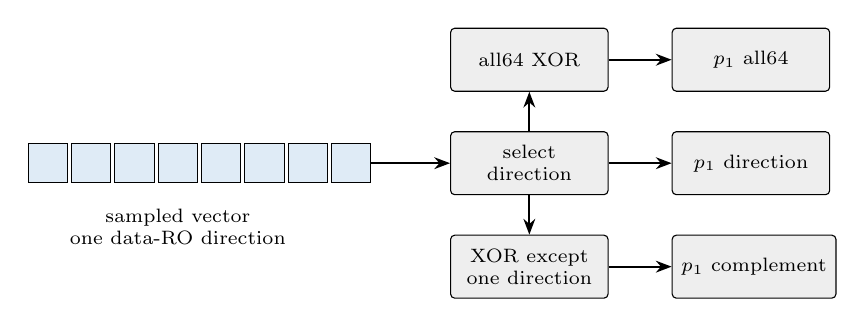
\begin{tikzpicture}[
  font=\scriptsize,
  bit/.style={draw, minimum width=5mm, minimum height=5mm, fill=softblue},
  block/.style={draw, rounded corners=1.5pt, minimum width=20mm, minimum height=8mm, align=center, fill=softgray},
  arr/.style={-{Stealth[length=2mm]}, thick}
]
\foreach \i in {0,...,7} {
  \node[bit] (b\i) at (\i*0.55,0) {};
}
\node[align=center, below=2mm of b3] {sampled vector\\one data-RO direction};
\node[block, right=10mm of b7] (select) {select\\direction};
\node[block, above=5mm of select] (all) {all64 XOR};
\node[block, below=5mm of select] (except) {XOR except\\one direction};
\draw[arr] (b7.east) -- (select.west);
\draw[arr] (select.north) -- (all.south);
\draw[arr] (select.south) -- (except.north);
\node[block, right=8mm of all] (p1a) {$p_1$ all64};
\node[block, right=8mm of select] (p1d) {$p_1$ direction};
\node[block, right=8mm of except] (p1e) {$p_1$ complement};
\draw[arr] (all) -- (p1a);
\draw[arr] (select) -- (p1d);
\draw[arr] (except) -- (p1e);
\end{tikzpicture}}
\caption{Reduced-XOR construction. The experiment compares the final all64 output, same-data-RO directions, complements that remove one direction from the final XOR, and line-direction controls that XOR across data ROs at one sampler phase.}
\label{fig:reducedxorconstruct}
\end{figure}

\begin{table*}[!t]
\centering
\caption{Complete reduced-XOR warmup-10 direction map. Run02 covers all eight same-data-RO directions and all eight complements; the all64 run02 row is retained as the corresponding final-output repeat context.}
\label{tab:reducedxor}
\scriptsize
\resizebox{\textwidth}{!}{%
\begin{tabular}{lllrrrrr}
\toprule
Mode & Direction & Label & $p_1$ r01 & Signed bias r01 & Min-H r01 & Worst $x$ r01 & $p_1$ r02 \\
\midrule
all64 & all & all64 & 0.458617 & -0.041383 & 0.885279 & 590 & 0.443194 \\
data\_ro & 0 & data\_ro0 & 0.191877 & -0.308123 & 0.307353 & 897 & 0.182267 \\
data\_ro & 1 & data\_ro1 & 0.518915 &  0.018915 & 0.946430 & 632 & 0.522621 \\
data\_ro & 2 & data\_ro2 & 0.244002 & -0.255998 & 0.403546 & 847 & 0.245911 \\
data\_ro & 3 & data\_ro3 & 0.671833 &  0.171833 & 0.573825 & 804 & 0.671545 \\
data\_ro & 4 & data\_ro4 & 0.424639 & -0.075361 & 0.797461 & 807 & 0.427625 \\
data\_ro & 5 & data\_ro5 & 0.409454 & -0.090546 & 0.759879 & 806 & 0.405413 \\
data\_ro & 6 & data\_ro6 & 0.375380 & -0.124620 & 0.678949 & 839 & 0.375746 \\
data\_ro & 7 & data\_ro7 & 0.549958 &  0.049958 & 0.862607 & 644 & 0.547275 \\
except\_data\_ro & 0 & except\_ro0 & 0.501020 &  0.001020 & 0.997060 & 571 & 0.500956 \\
except\_data\_ro & 1 & except\_ro1 & 0.550312 &  0.050312 & 0.861678 & 597 & 0.553538 \\
except\_data\_ro & 2 & except\_ro2 & 0.499674 & -0.000326 & 0.999060 & 557 & 0.499543 \\
except\_data\_ro & 3 & except\_ro3 & 0.553930 &  0.053930 & 0.852224 & 603 & 0.553217 \\
except\_data\_ro & 4 & except\_ro4 & 0.520205 &  0.020205 & 0.942848 & 570 & 0.519451 \\
except\_data\_ro & 5 & except\_ro5 & 0.565521 &  0.065521 & 0.822347 & 620 & 0.566377 \\
except\_data\_ro & 6 & except\_ro6 & 0.501833 &  0.001833 & 0.994721 & 556 & 0.500471 \\
except\_data\_ro & 7 & except\_ro7 & 0.542602 &  0.042602 & 0.882034 & 598 & 0.542643 \\
\bottomrule
\end{tabular}}
\end{table*}

\begin{table*}[!t]
\centering
\caption{Reduced-XOR mechanism controls. The full-direction repeat tests run-to-run stability of the warmup-10 direction map; the second-board rows test cross-board mechanism persistence; the line-direction rows test whether warmup-10 bias is a sampler-phase row failure; the data\_ro3 warmup-neighbor rows test whether the strongest high-biased direction is unique to warmup 10.}
\label{tab:reducedxormechanism}
\scriptsize
\begin{tabular}{@{}L{0.20\textwidth}L{0.25\textwidth}L{0.25\textwidth}L{0.22\textwidth}@{}}
\toprule
Control & Measured scope & Key values & Mechanism reading \\
\midrule
Warmup-10 same-data-RO directions & eight $y_{\mathrm{ro}i}$ rows & $p_1$ range 0.191877--0.671833; max abs bias 0.308123; min min-H 0.307353 & Strong anisotropy along same-data-RO directions \\
Warmup-10 full direction repeat & eight $y_{\mathrm{ro}i}$ and eight $y_{\mathrm{except}\ i}$ rows in run01/run02 & data\_ro Pearson 0.999678, mean $|\Delta p_1|=0.003199$, same sign 8/8; complements Pearson 0.999013, mean $|\Delta p_1|=0.000893$, same sign 8/8 & Repeat-stable anisotropic direction map at warmup 10 \\
Second-board full direction maps & warmup-10 and warmup-11 all64, data\_ro0..7, and except\_ro0..7 & W10 all64 $p_1=0.360614$; except\_ro0, except\_ro2, except\_ro6 near balanced at 0.500015, 0.502798, 0.500649; W11 all64 $p_1=0.473738$ & Same cancellation mechanism appears on a second board, but contributor identities and magnitudes are board specific \\
Warmup-10 sampler-phase line directions & eight $y_{\mathrm{line}k}$ rows & $p_1$ range 0.486473--0.501004; max abs bias 0.013527; min min-H 0.961488 & No evidence of a generic sampler-phase line failure in this run \\
Line6 targeted repeat & $y_{\mathrm{line}6}$ run01 and repeat02 & $p_1=0.486473$ and 0.487182; worst byte.bit remains 0.3; worst $x=701$ and 714 & Stable fixed-position outlier with weak global bias \\
data\_ro3 warmup neighbors & $y_{\mathrm{ro}3}$ and except\_ro3 at warmups 5, 10, 11 & data\_ro3 $p_1=0.576638$, 0.671833, 0.544560; except\_ro3 $p_1=0.503005$, 0.553930, 0.501558 & Direction persists; complement cancellation is warmup-dependent \\
\bottomrule
\end{tabular}
\end{table*}

\begin{figure}[t]
\centering
\resizebox{\columnwidth}{!}{%
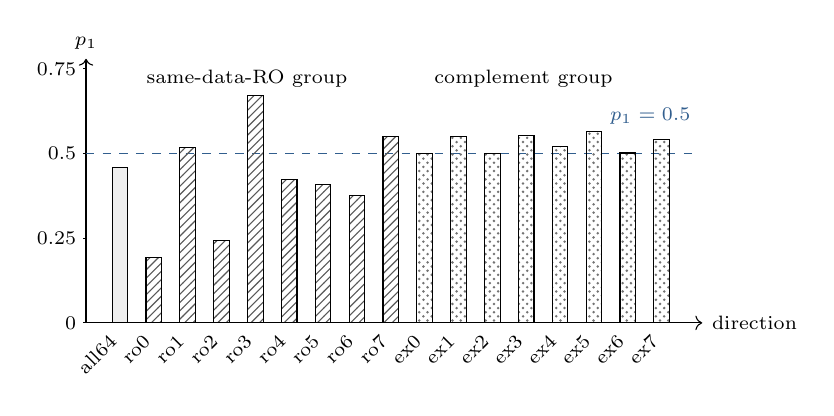
\begin{tikzpicture}[font=\scriptsize, x=0.43cm, y=4.3cm]
\draw[->] (0,0) -- (18.2,0) node[right] {direction};
\draw[->] (0,0) -- (0,0.78) node[above] {$p_1$};
\foreach \y/\lab in {0/0,0.25/0.25,0.5/0.5,0.75/0.75} {
  \draw (-0.08,\y) -- (0,\y) node[left] {\lab};
}
\draw[dashed, boundaryblue] (0,0.5) -- (18.0,0.5);
\draw[fill=softgray, draw=black] (0.77,0) rectangle (1.23,0.458617);
\draw[fill=softorange, pattern=north east lines, pattern color=black!65, draw=black] (1.77,0) rectangle (2.23,0.191877);
\draw[fill=softorange, pattern=north east lines, pattern color=black!65, draw=black] (2.77,0) rectangle (3.23,0.518915);
\draw[fill=softorange, pattern=north east lines, pattern color=black!65, draw=black] (3.77,0) rectangle (4.23,0.244002);
\draw[fill=softorange, pattern=north east lines, pattern color=black!65, draw=black] (4.77,0) rectangle (5.23,0.671833);
\draw[fill=softorange, pattern=north east lines, pattern color=black!65, draw=black] (5.77,0) rectangle (6.23,0.424639);
\draw[fill=softorange, pattern=north east lines, pattern color=black!65, draw=black] (6.77,0) rectangle (7.23,0.409454);
\draw[fill=softorange, pattern=north east lines, pattern color=black!65, draw=black] (7.77,0) rectangle (8.23,0.375380);
\draw[fill=softorange, pattern=north east lines, pattern color=black!65, draw=black] (8.77,0) rectangle (9.23,0.549958);
\draw[fill=softblue, pattern=crosshatch dots, pattern color=black!55, draw=black] (9.77,0) rectangle (10.23,0.501020);
\draw[fill=softblue, pattern=crosshatch dots, pattern color=black!55, draw=black] (10.77,0) rectangle (11.23,0.550312);
\draw[fill=softblue, pattern=crosshatch dots, pattern color=black!55, draw=black] (11.77,0) rectangle (12.23,0.499674);
\draw[fill=softblue, pattern=crosshatch dots, pattern color=black!55, draw=black] (12.77,0) rectangle (13.23,0.553930);
\draw[fill=softblue, pattern=crosshatch dots, pattern color=black!55, draw=black] (13.77,0) rectangle (14.23,0.520205);
\draw[fill=softblue, pattern=crosshatch dots, pattern color=black!55, draw=black] (14.77,0) rectangle (15.23,0.565521);
\draw[fill=softblue, pattern=crosshatch dots, pattern color=black!55, draw=black] (15.77,0) rectangle (16.23,0.501833);
\draw[fill=softblue, pattern=crosshatch dots, pattern color=black!55, draw=black] (16.77,0) rectangle (17.23,0.542602);
\node[rotate=45, anchor=east] at (1,-0.025) {all64};
\node[rotate=45, anchor=east] at (2,-0.025) {ro0};
\node[rotate=45, anchor=east] at (3,-0.025) {ro1};
\node[rotate=45, anchor=east] at (4,-0.025) {ro2};
\node[rotate=45, anchor=east] at (5,-0.025) {ro3};
\node[rotate=45, anchor=east] at (6,-0.025) {ro4};
\node[rotate=45, anchor=east] at (7,-0.025) {ro5};
\node[rotate=45, anchor=east] at (8,-0.025) {ro6};
\node[rotate=45, anchor=east] at (9,-0.025) {ro7};
\node[rotate=45, anchor=east] at (10,-0.025) {ex0};
\node[rotate=45, anchor=east] at (11,-0.025) {ex1};
\node[rotate=45, anchor=east] at (12,-0.025) {ex2};
\node[rotate=45, anchor=east] at (13,-0.025) {ex3};
\node[rotate=45, anchor=east] at (14,-0.025) {ex4};
\node[rotate=45, anchor=east] at (15,-0.025) {ex5};
\node[rotate=45, anchor=east] at (16,-0.025) {ex6};
\node[rotate=45, anchor=east] at (17,-0.025) {ex7};
\node[anchor=east, text=boundaryblue, fill=white, inner sep=1pt] at (17.95,0.61) {$p_1=0.5$};
\node[anchor=west] at (1.5,0.72) {same-data-RO group};
\node[anchor=west] at (10.0,0.72) {complement group};
\end{tikzpicture}}
\caption{Warmup-10 reduced-XOR $p_1$ values for the complete run01 direction map. The left group contains all64 followed by same-data-RO directions; the right group contains complements. Bar patterns distinguish the groups for grayscale viewing.}
\label{fig:reducedxor}
\end{figure}

The mechanism controls in Table~\ref{tab:reducedxormechanism} sharpen the interpretation. The warmup-10 sampled vector is strongly anisotropic and repeat-stable: across the complete run01/run02 direction map, same-data-RO directions have Pearson correlation 0.999678 in $p_1$, mean absolute run-to-run change 0.003199, and the same bias sign in all eight directions. The complement directions show the same qualitative stability with Pearson correlation 0.999013, mean absolute change 0.000893, and matching bias signs in all eight directions. In contrast, sampler-phase line directions remain close to balance, spanning $p_1=0.486473$ to 0.501004. Thus the dominant marginal reduced-XOR structure in this run is not a generic failure of one sampler phase line. It is concentrated in same-data-RO directions and then reshaped by XOR complements.

The second-board reduced-XOR check reinforces this mechanism without implying identical board behavior. At warmup 10, the second-board all64 output is biased low ($p_1=0.360614$), while removing data\_ro0, data\_ro2, or data\_ro6 nearly balances the stream ($p_1=0.500015$, 0.502798, and 0.500649). At warmup 11, all64 moves closer to balance ($p_1=0.473738$), but individual same-data-RO contributors remain strongly biased; near-balanced removal cases shift to except\_ro3, except\_ro6, and except\_ro1. This is consistent with the same warmup-dependent signed-contributor model observed on the primary board, with board-specific contributor identities and magnitudes.

The data\_ro3 warmup-neighbor control further shows that the strongest high-biased warmup-10 direction is not a one-run anomaly. It remains high-biased at warmups 5, 10, and 11, but the except\_ro3 complement is near balanced at warmups 5 and 11 and moderately high-biased at warmup 10. This supports a warmup-dependent complement-cancellation model: individual same-data-RO directions can be stable biased hardware functions, while final all64 quality depends on how the remaining directions cancel or reinforce them under a specific startup window. The line6 repeat gives a different pattern: weak global bias but a stable worst fixed-position outlier, consistent with fixed-position startup structure rather than a row-direction analogue of the strong data-RO direction bias.

Taken together, these measurements reinforce the sampler-boundary argument. The measured output is shaped by a vector of sampler-side hardware functions and startup-dependent XOR interactions, not only by a single abstract data-RO entropy term.

\section{Entropy-Source Boundary Discussion}

The evidence chain supports a bounded physical boundary claim. Placement experiments show that implementation choices materially affect continuous-stream statistics. Restart experiments show that continuous-stream quality is not sufficient to characterize startup behavior. The primary-board sampler-side counterfactuals show that changing sample-RO physical implementation can move measured restart outcomes in both directions, and the targeted second-board counterfactual reproduces the same direction of sampler-lock effect with board-specific magnitude. Pairwise and reset-aligned \tdc{} diagnostics constrain one simple mechanism story, and reduced-XOR experiments show that final output quality can reflect same-data-RO direction anisotropy and warmup-dependent complement cancellation across both measured boards.

Taken together, these results support treating sampler-side physical implementation as part of the measured entropy-source boundary. In this work, that boundary includes the data ROs, sampled-data registers, sample RO, sampler-side routing, and restart/warmup/reset timing that directly determines early-sampling behavior. Post-XOR FIFO buffering, UART transport, host capture, and offline scripts are part of the measurement/readout chain, not the entropy-source boundary. Their routed movement in the current diff is therefore treated as a residual confounder to audit, not as a reason to include the whole bitstream in the entropy source.

The interpretation is narrower than a proof of root cause. The measurements do not show that all sampler-side elements contribute equally, and they do not define a validated placement-aware design rule. They do show that excluding the sampler side from the measured boundary would hide a physical implementation factor that can substantially reshape restart outcomes in the evaluated implementations.

For measurement practice, the consequence is direct. An FPGA \rotrng{} evaluation should report not only final output statistics, but also the physical sampler implementation, restart behavior, and diagnostic evidence that separates data-RO behavior from sampler-vector and readout effects. Where possible, counterfactual placements should be used to test whether a claimed entropy-source boundary is stable under small physical changes.

\section{Limitations and Future Measurements}

The first limitation is scope. The evidence now includes a primary Zynq-7020 board and a targeted second same-family board check, but it is still not a broad multi-board validation. Cross-family, larger board-count, voltage, temperature, aging, and tool-version evidence would be required before making broader implementation rules.

The second limitation is standards interpretation. The project contains 8,000,000-symbol entropy-assessment summaries and 1000-row restart diagnostic evidence, but a complete validation package would also require a final component boundary, conditioning and health-test documentation, restart-equivalence argument, environmental evidence, and submission-ready traceability.

The third limitation is \tdc{} interpretation. Pairwise and clean reset-aligned \tdc{} measurements are useful diagnostic evidence, and code-density calibration supports cautious use, but the current calibration does not justify absolute picosecond-level jitter or phase-noise claims.

The fourth limitation is physical decomposition. The sampler-side counterfactual localizes the intended perturbation to sample-RO physical constraints, and the same-RTL forward audit keeps tracked data-RO cells and sampled-data registers fixed at the LOC/BEL level. It still does not exhaustively separate sample-RO stages, local routes, post-XOR FIFO interaction, reset sequencing, or placement-neighborhood effects. Existing resource, timing, power, route-status, routed-cell, routed-net, PIP, net-delay, and directive-controlled route-variance reports provide traceability for the implemented variants; a route-locked repeat would make the physical attribution stronger.

The highest-priority future measurements are additional same-family boards, controlled PVT subsets, held-out sampler placements, \tdc{} captures around the strongest counterfactuals, and route-locked repeats for the locked-sampler designs. For the reduced-XOR mechanism, full all-direction repeats at warmups 5 and 11 on the primary board and additional second-board repeats would test how far the observed contributor-cancellation model generalizes. With such evidence, the same core result could later be compressed toward a circuits-and-systems contribution, expanded toward a VLSI implementation rule, or reframed around a more complete cryptographic-engineering validation boundary.

\section{Conclusion}

This paper presented a measurement-driven two-board diagnosis of sampler-side entropy boundaries in Zynq-7020 FPGA \rotrng{}s. Continuous-stream measurements show strong placement dependence on the primary board, restart measurements reveal fixed-position startup bias that continuous-stream balance does not capture, and sampler-side counterfactuals show that a sampler-centered physical perturbation with entropy-source-local routed-network residuals can move restart behavior from near balance to flagged bias and back toward near balance on the primary board, with the same sampler-lock direction reproduced in targeted second-board checks.

The supporting diagnostics make the claim more specific. Pairwise and exact counterfactual \tdc{} measurements do not support a simple persistent hard-locking-only explanation under the selected conditions, and reduced-XOR counterfactuals show that final all64 output can hide biased internal sampler-vector directions through warmup-dependent cancellation on both measured boards. The resulting conclusion is a measurement and diagnosis claim: in the evaluated implementations, sampler-side physical implementation should be included in the measured entropy-source boundary.

\bibliographystyle{IEEEtran}
\bibliography{../refs/references}

\end{document}
